\documentclass[a4paper, 12pt, fleqn]{article}
\usepackage{libertine}
% \usepackage{setspace}%\setstretch{1.24} %Zeilenabstand �ndern
\usepackage[utf8]{inputenc} %Umlaute&Sonderzeichen einlesbar
\usepackage[normalem]{ulem}
\usepackage{amsmath,amssymb,amsthm}
\theoremstyle{definition}
\newtheorem{hyp}{H} 
\usepackage{natbib}
\setcitestyle{notesep={; }}

\usepackage[pdfborder={0 0 0}, breaklinks=true]{hyperref}
\usepackage{microtype}
\usepackage{booktabs}
\usepackage{graphicx}
\usepackage{pdflscape}
\usepackage{float}
\usepackage{pdfpages}
\usepackage{floatflt}
\long\def\symbolfootnote[#1]#2{\begingroup%
\def\thefootnote{\fnsymbol{footnote}}\footnote[#1]{#2}\endgroup}
\usepackage{array}
\newcommand{\inew}[1]{{\color{blue} #1\color{black}}}
\usepackage{comment}
\specialcomment{icomm}{\color{red}\footnotesize [\textsc{iren}: }{] \normalsize\color{black}}
\newcommand{\iout}[1]{{\color{red}\sout{#1}}}
%}
\newcommand{\old}[1]{{\color{lightgray} #1\color{black}}}

\newcommand{\mytitle}{{\Large \textsc{When personalization deters delegation to algorithms: Evidence from a preregistered experiment}}}

%opening
\title{\mytitle}
%\author{Wania Lefuloff}
\date{}

%Fuer Zeilenabstand
\usepackage{setspace}
%\doublespacing

%Fuer 1.5 inch margins
%\usepackage[a4paper]{geometry}
%\geometry{top=1.5in, bottom=1.5in, left=1.2in, right=1.2in}

\begin{document}
 
%  \maketitle
\thispagestyle{empty}
\begin{center}
  \mytitle\symbolfootnote[4]{We are grateful to all the many people who helped us write this paper, first and foremost Chris Starmer and Robin Cubitt, to whom we owe several aspects of the design, as well as the lively research group at the TWI and participants of numerous workshops and conferences.}
  \vspace{.55cm}\\
 Lara Suraci \qquad\qquad\qquad Irenaeus Wolff\symbolfootnote[3]{Corresponding author. Thurgau Institute of Economics, Hafenstrasse 6, 8280 Kreuzlingen, Switzerland, \textit{wolff@twi-kreuzlingen.ch}.}
\\\vspace{.25cm}
 \begin{small}
  \phantom{mortext}\textit{DG Cities \qquad\qquad Thurgau Institute of Economics \\ \phantom{moretext}\phantom{University} \qquad\qquad (TWI) / University of Konstanz} %University of Konstanz\\ Hafenstrasse 6, 8280 Kreuzlingen, Switzerland\\ wolff@twi-kreuzlingen.ch}
  \vspace{.03cm}\\
\vspace{.6cm}
 {This version: 23$^{\text{rd}}$ March, 2026}
\vspace{.6cm}
\end{small}
\end{center}

\begin{abstract}
  Algorithmic decision aids increasingly act on users’ behalf, and in many instances users can either retain control or delegate decisions to an algorithm. We test whether preference-based personalization increases or decreases willingness to delegate compared with an objective optimization criterion. In a preregistered between-subjects experiment (N = 233), participants repeatedly chose whether to decide themselves or to delegate to an algorithm. In one treatment, the delegation option is an optimization-based algorithm selecting the option with the highest expected value. In the other treatment, it is a preference-based (personalized) algorithm selecting according to participants’ previously elicited preferences. We find no evidence that preference-based personalization increases delegation relative to expected-value optimization throughout the task. Instead, personalization deters delegation in two ways. First, at first contact participants are significantly less likely to delegate to the preference-based algorithm than to the optimization-based algorithm; this difference is confined to the very first decision and disappears immediately thereafter, with delegation rates statistically indistinguishable across algorithm types in subsequent decisions. Second, categorical non-delegation (never delegating) is substantially more prevalent under preference-based personalization (15.7\%) than under objective optimization (3.4\%). 
  Taken together, the results are consistent with the idea that preference-matching can raise initial hesitation and heighten agency- and responsibility-related concerns for a subset of users, functioning as an acceptance barrier even when personalization is normatively appealing.
  
     \vspace{.25cm}
  \textit{Keywords:} {AI delegation, human-AI delegation, personalization, algorithm appreciation, algorithm aversion, trust in AI, financial decision-making, preregistered experiment.}\vspace{.15cm}
  \\\textit{JEL:} {D81, C91, D83}
\end{abstract}
\vspace{-.5cm}

\section{Introduction}\label{sec:intro}
Algorithmic systems increasingly make and implement decisions on users’ behalf in both everyday and high-stakes contexts, from automated driving and financial robo-advising to autonomous trading and smart-home control. Public perceptions of algorithmic decision-making vary substantially across domains and are shaped by perceived legitimacy and accountability \citep{Aysolmaz2023}. In many such settings, users face a concrete choice: they can retain control and decide themselves, or delegate the decision to an algorithm. Delegation can reduce cognitive effort and simplify complex choice tasks, but it can also reshape perceived agency and responsibility for outcomes. Recent literature shows that people do delegate consequential choices to AI systems, yet such delegation is psychologically nuanced and sensitive to characteristics of the decision maker \citep{Candrian2022}. Throughout the paper, we use the term ``algorithmic decision aid'' broadly to include both rule-based algorithms and AI-based systems. This reflects the practical reality that, from a user's perspective, the boundary between ``AI'' and other algorithmic decision rules is often opaque.

A common assumption is that \emph{personalization} should increase acceptance. If individuals differ in preferences, then a decision aid that incorporates those preferences should, in principle, deliver higher subjective utility than a one-size-fits-all rule. In financial decision support, for example, systems often elicit risk preferences and map them to recommended portfolios; acceptance of robo-advisory tools has therefore been studied through standard adoption lenses \citep{Figa-Talamanca2022,Mahmud2025}.
\begin{icomm}
	 check final sentence/lit in there
\end{icomm}

However, behavioral evidence suggests that willingness to use algorithmic advice is not determined by instrumental considerations alone. People sometimes avoid algorithms and sometimes prefer them, depending on context and perceived role \citep{Dietvorst2018,Logg2019}. They also interpret and rationalize recommendations rather than mechanically follow them \citep{Yeomans2019}, and interdisciplinary syntheses emphasize that acceptance depends on multiple moderators \citep[including perceived control;][]{Mahmud2022,Chugunova2022}. 

Preference-based personalization can therefore be double-edged: while it promises better fit, it can also make decisions traceable to a user profile, potentially heightening discomfort with being categorized or increasing perceived responsibility for outcomes (``it chose based on me'').
\begin{icomm}
	Include somewhere that this doesn't seem to be the case in our case, as wanting to be responsible for the outcome is often-cited among the non-delegators
\end{icomm}
 Consistent with this, recent evidence shows that increased transparency can backfire by triggering negative social interpretations and reducing acceptance \citep{Chen2024}, and that transparency can produce resistance rather than compliance in algorithmic management contexts \citep{Hu2024}. Related work further argues that acceptance of automated decision-making depends less on whether the system is an ``agent'' and more on perceived benefits and control \citep{Schaap2024}.

These issues are especially salient at {first contact}, when users have no experiential basis for evaluating an algorithm. In repeated interaction settings, people can quickly settle into stable interaction strategies, and overreliance (and its costs) can emerge even when performance information is available \citep{Klingbeil2024}. Moreover, reactions to algorithmic errors can be robust
\begin{icomm}
	"robust"?
\end{icomm} 
\citep{Renier2021}, suggesting that expectations about how an algorithm will behave may matter disproportionately early on. Importantly, behavioral reliance and self-reported trust need not coincide: evidence from AI-advisor interactions shows that determinants of behavioral trust can diverge from self-reported trust \citep{Schreibelmayr2025}. 
\begin{icomm}
	This seems like trying to say that our study has an advantage over certain other studies, but I'm not sure this is the most elegant way nor the best place in the paper to say this. Ah, I get the answer to the second point: it's here to make the statement "Together, ..." in the subsequent paragraph. 
\end{icomm}

Finally, autonomy considerations are themselves a driver of acceptance: increasing user autonomy can increase recommendation acceptance \citep{Fink2024}, and preferences for decision autonomy can constrain delegation even when delegation is instrumentally attractive \citep{Ivanova-Stenzel2025}. Together, this motivates studying delegation as an observable behavior and treating first contact as a critical moment when abstract cues about an algorithm's decision logic may dominate.

In this study, we contrast two decision rules that are both plausible in financial choice settings but may elicit different reactions. One algorithm follows an \emph{objective optimization rule} and selects the option with the highest expected value (EV), which may appear impersonal and easier to justify as an external computation. 
\begin{icomm}
	"as an external computation"?
\end{icomm}
The other is \emph{preference-based personalization} in a narrow sense: it selects options according to participants' previously elicited (revealed) preferences rather than by optimizing EV. Here, ``personalized'' refers to profile-based selection from elicited preferences, not to online learning or continuous adaptation. 
\begin{icomm}
	I get the contrast, but is this the best way to describe our algorithm? The algorithm is really trivial: it chooses the same option that the participant had chosen in an `easier' environment in a prior part of the experiment (no time pressure, no additional but dominated options, no mixing of states of nature to make it harder to compare lotteries...).
\end{icomm}
The central question is whether people are more willing to delegate to EV maximization than to preference-based personalization. This comparison also connects to work showing that delegation can serve responsibility-sharing motives \citep{Kirchkamp2019} 
\begin{icomm}
	also Werner, Suraci, and Wolff (working paper), in a context that is closer to the one used in this paper
\end{icomm}
and to recent studies on blame dynamics and delegation in financial contexts \citep{Ismagilova2025}.
\begin{icomm}
	rephrase ("blame dynamics" is not very clear)
\end{icomm}

\subsection*{Preregistered hypothesis and analysis plan}
Consistent with our preregistration ({\footnotesize\url{https://aspredicted.org/7un5qf.pdf}}), the main hypothesis is: 
\begin{hyp}
	People are more likely to delegate financial decisions to an EV-maximizing algorithm than to a personalized algorithm that incorporates their (revealed) preferences.
\end{hyp}

Our preregistered primary analyses test this hypothesis in two complementary ways. First, we test the treatment difference in delegation in the first decision (round 1) using a one-sided Boschloo exact test. This isolates first contact, when participants have no outcome feedback and must decide whether to delegate based on their interpretation of the algorithm. Second, we test whether EV maximization leads to higher delegation overall by comparing participants' average delegation frequencies across rounds using a one-sided Wilcoxon--Mann--Whitney test.

To account for the repeated-decision structure and additional determinants of delegation, our preregistration also specifies a multivariate regression analysis. We estimate a model with treatment indicators interacted with the decision period, decision-ID fixed effects, and participant-clustered standard errors. We further include the feedback history in the form of including the share of zero outcomes among prior delegated choices, to control for how experienced payoffs may influence subsequent delegation decisions. This preregistered specification tests whether any treatment difference varies systematically over decisions while controlling for option-set heterogeneity and participants' feedback histories.

\subsection*{Study overview and supplementary analyses}
We implement this design in a preregistered between-subjects experiment in which participants repeatedly choose whether to decide themselves or delegate to the assigned algorithm. The repeated-decision setting provides a direct behavioral measure of delegation and allows us to distinguish first-contact delegation from later decisions made after minimal experience.

In addition to the preregistered tests, we report a small set of analyses to characterize heterogeneity in delegation propensity. In particular, we examine categorical non-delegation (never delegating across rounds). This outcome captures a distinct form of resistance to algorithmic control transfer and is relevant for understanding which users may opt out of decision aids altogether.

In sum, this paper provides a preregistered test of a simple but consequential claim: even in a setting where preference-based personalization may appear normatively attractive, people may nonetheless be more willing to delegate to a `more objective' algorithm. Our design and preregistered analyses allow us to assess this claim both at first contact and on average across repeated decisions, and show that resistance to personalization can take the form of both first-contact hesitation and categorical non-delegation.




%A common assumption is that personalization should increase acceptance. If individuals differ in preferences, then a decision aid that incorporates those preferences should, in principle, deliver higher subjective utility than a one-size-fits-all rule. In financial decision support, for example, systems often elicit risk preferences and map them to recommended portfolios. However, behavioral evidence suggests that willingness to use algorithmic advice is not determined by instrumental considerations alone. People sometimes avoid algorithms, sometimes prefer them, and often react to how they interpret a system’s role and legitimacy (e.g., Dietvorst et al., 2015; Logg et al., 2019; Castelo et al., 2019). Preference-based personalization can therefore be double-edged: while it promises better fit, it can also make the system’s decisions traceable to a user profile, potentially heightening discomfort with being categorized or increasing perceived responsibility for outcomes (“it chose based on me”).
%
%These issues are especially salient at first contact, when users have no experiential basis for evaluating an algorithm. At first contact, delegation is likely to depend on abstract cues about what an algorithm optimizes and what that implies about the user, rather than on experienced accuracy. Therefore, early impressions and system descriptions can shape adoption and reliance even when objective performance is held constant (e.g., Kosch et al., 2022). Moreover, self-reported trust and behavioral reliance often diverge (Papenmeier et al., 2022), which motivates studying delegation as an observable behavior rather than equating it with stable trust. 
%
%In this study, we contrast two decision rules that are both plausible in financial choice settings but may elicit different reactions. One algorithm selects the option with the highest expected value (EV), a rule that may appear impersonal and objectively justified. The other is preference-based (“personalized”) in a narrow sense: it selects options according to participants’ previously elicited (revealed) preferences rather than by optimizing EV. Here, “personalized” refers to profile-based selection from elicited preferences, not to online learning or continuous adaptation. The central question is whether people are more willing to delegate to EV maximization than to preference-based personalization.
%
%Preregistered hypothesis and analysis plan
%
%Consistent with our preregistration, the main hypothesis is:
%
%H1 (Preregistered). People are more likely to delegate financial decisions to an EV-maximizing algorithm than to a personalized algorithm that incorporates their (revealed) preferences.
%
%Our preregistered primary analyses test this hypothesis in two complementary ways. First, we test the treatment difference in delegation in the first decision (round 1) using a one-sided Boschloo exact test. This isolates first contact, when participants have no outcome feedback and must decide whether to delegate based on their interpretation of the algorithm. Second, we test whether EV maximization leads to higher delegation overall by comparing participants’ average delegation frequencies across rounds using a one-sided Wilcoxon–Mann–Whitney test.
%
%To account for the repeated-decision structure and additional determinants of delegation, our preregistration also specifies multivariate regression analyses. We estimate models with treatment indicators interacted with the decision period, decision-ID fixed effects, and participant-clustered standard errors. We further include measures capturing feedback history, including the share of zero outcomes among prior delegated choices, to control for how experienced payoffs may influence subsequent delegation decisions. This preregistered specification tests whether any treatment difference varies systematically over decisions while controlling for option-set heterogeneity and participants’ feedback histories.
%
%Study overview and supplementary analyses
%
%We implement this design in a preregistered between-subjects experiment in which participants repeatedly choose whether to decide themselves or delegate to the assigned algorithm. The repeated-decision setting provides a direct behavioral measure of delegation and allows us to distinguish first-contact delegation from later decisions made after minimal experience.
%
%In addition to the preregistered tests, we report a small set of analyses to characterize heterogeneity in delegation propensity. In particular, we examine categorical non-delegation (never delegating across rounds). This outcome captures a distinct form of resistance to algorithmic control transfer and is relevant for understanding which users may opt out of decision aids altogether. 
%
%In sum, this paper provides a preregistered test of a simple but consequential claim: even in a setting where preference-based personalization may appear normatively attractive, people may nonetheless be more willing to delegate to an EV-maximizing algorithm. Our design and preregistered analyses allow us to assess this claim both at first contact and on average across repeated decisions, and show that resistance to personalization can take the form of both first-contact hesitation and categorical non-delegation.


\section{Related Work}
\label{sec:related}

Our work sits at the intersection of literatures on (i) behavioral uptake of algorithmic decision aids, (ii) delegation and responsibility in human--algorithm interaction, and (iii) personalization and transparency as acceptance levers that may also create resistance. Below, we situate our preregistered comparison of an EV-maximizing algorithm versus a preference-based (personalized) algorithm within these streams.

\subsection{Algorithm aversion, appreciation, and conditions for uptake}
A central starting point is the mixed evidence on whether people follow algorithmic advice. Seminal work on \emph{algorithm aversion} shows that people may avoid algorithms after observing them err, even when the algorithm performs well in expectation \citep{Dietvorst2018}. Subsequent research documents also cases of \emph{algorithm appreciation} (in which people prefer algorithmic to human judgment) and highlights that adoption depends on context and comparison standards \citep{Logg2019}. In addition, people actively interpret and rationalize recommendations, which can affect whether they use them and how they integrate them with their own judgment \citep{Yeomans2019}. A recent systematic review synthesizes this body of work and emphasizes moderators that shape the direction and magnitude of aversion/appreciation effects \citep{Mahmud2022}. More broadly, an interdisciplinary review of experiments on human--machine interaction provides additional integration across disciplinary boundaries and underscores how acceptance depends on what the machine is perceived to be doing and for whom \citep{Chugunova2022}. 
\begin{icomm}
	check: is this truly broader? Is Mahmud et al. not interdisciplinary?
\end{icomm}
Together, this literature motivates our focus on a concrete behavioral outcome---delegation---and on how the \emph{decision rule} (objective EV maximization vs preference-based personalization) shapes willingness to hand over control to an algorithm.

\subsection{Delegation, agency, and responsibility sharing}
Delegation differs from merely receiving advice: it is a choice to transfer control to another actor (here, an algorithm) and is therefore closely tied to perceived agency and responsibility. Empirical work on delegation to autonomous AI demonstrates that people do not only consider expected payoffs; they also weigh the interactional meaning 
\begin{icomm}
	"weigh the interactional meaning" has to be decoded
\end{icomm}
of handing over a decision \citep{Candrian2022}. Complementing this, work on responsibility sharing suggests that decision-makers may strategically value distributing or externalizing accountability to a machine \citep{Kirchkamp2019}. Related studies in organizational and leadership contexts similarly show that perceptions of legitimacy, competence, and responsibility affect acceptance of algorithmic decision-makers \citep{Hoeddinghaus2021}. Recent work on choosing between human and algorithmic advisors further points to responsibility sharing as a key determinant of advisor choice \citep{Gazit2023}. A complementary perspective comes from work on \emph{human-in-the-loop} designs: allowing human involvement can increase uptake but may reduce decision accuracy, underlining that control allocation shapes behavior and outcomes \citep{Sele2024}. Finally, preference for decision autonomy has been theorized and empirically examined as a stable individual tendency that can constrain algorithm adoption, even when delegation is instrumentally attractive 
\begin{icomm}
	"instrumentally attractive" has to be decoded
\end{icomm}
\citep{Ivanova-Stenzel2025}. These strands provide a natural backdrop for our preregistered hypothesis that delegation may be higher for an impersonal, EV-maximizing rule than for a preference-based rule that implicates the self.
\begin{icomm}
	"implicates the self" has to be decoded
\end{icomm}

\subsection{Personalization as an acceptance lever---and as a potential barrier}
Personalization is often assumed to increase acceptance by aligning system behavior with users' preferences. However, several streams suggest that personalization can also create resistance by increasing perceived self-relevance, profiling concerns, or accountability. In algorithmic recommendation settings, opening the ``black box'' can backfire when it induces meta-level social interpretations (e.g., feelings of being judged or dehumanized), which in turn reduce acceptance \citep{Chen2024}. Work on algorithmic management similarly points to a {transparency--resistance paradox}, showing that more visibility into algorithmic logic 
\begin{icomm}
	"visibility into algorithmic logic" has to be decoded
\end{icomm}
can sometimes increase pushback rather than compliance \citep{Hu2024}. 
\begin{icomm}
	Doesn't this belong to the next subsection (on Transparency, explainability...)?
\end{icomm}
In addition, recent work emphasizes that acceptance is shaped less by whether a system is an ``agent'' per se and more by perceived benefits and {control}, directly relevant to our interpretation of preference-based personalization as potentially reducing perceived autonomy \citep{Schaap2024}. 
\begin{icomm}
	not sure about the wording. First, I think "potentially reducing" is not the right word, but maybe "threatening" could be. In addition, the EV-algorithm could be seen as "more controlled" in the sense that people might feel that they know less about what the personalized algorithm does, which is a different argument, however.
\end{icomm}
These findings resonate with our focus on preference-based decision rules as a special case of personalization: even if normatively appealing, preference-based selection may feel more self-representational 
\begin{icomm}
	is that plausible? That people feel represented better and therefore resist more? I wouldn't think so. I do buy the story of the autonomy threat (and the loss of control, which also seems to be a central element of the next subsection; should 2.3 and 2.4 be merged?)
\end{icomm}
and thus be resisted by some users.

\subsection{Transparency, explainability, and reliance behavior}
A large literature studies whether transparency and explainability increase trust, reliance, and compliance with AI outputs. The ``algorithmic affordance'' perspective emphasizes fairness, accountability, and transparency as drivers of how users interpret and engage with algorithmic systems \citep{Shin2019}. Experimental work shows that explainable AI can shift both trust and behavior, especially in higher-stakes decision tasks \citep{Leichtmann2023}. Work on decision control and explanations in human--AI collaboration finds that giving users more control (and appropriately designed explanations) can improve perceptions and compliance \citep{Westphal2023}. In applied decision-support contexts, transparency affects advice utilization through psychological mediators such as trusting beliefs and perceived understanding \citep{Ning2024}. Importantly, transparency effects may depend on whether system performance meets expectations: when outcomes confirm expectations, transparency can play a different role than when they do not \citep{Sun2026}. These findings motivate our preregistered modeling choices 
\begin{icomm}
	how about "analysis"?
\end{icomm}
that account for feedback histories (e.g., the share of zero outcomes among prior delegated choices) and decision periods, because experienced outcomes are a central driver of subsequent reliance.

\subsection{Contextual and individual-difference moderators of trust and delegation}
Recent work increasingly emphasizes heterogeneity: algorithm uptake varies across people, tasks, and situational constraints. An experimental study of overreliance documents both the extent and the potential costs of relying too heavily on AI \citep{Klingbeil2024}. Complementing this, research on user autonomy shows that allowing users to decide can increase acceptance of recommendations, suggesting that autonomy concerns can be a primary driver of behavior \citep{Fink2024}. Personality and context also shape delegation and collaboration with algorithms \citep{Ferraz2025}. Task properties matter as well: trust and reliance vary with task objectivity, time pressure, and cognitive load \citep{Yang2025}. More generally, psychological readiness has been proposed as a determinant of whether people are willing to accept algorithmic advice at all \citep{Kim2026}. Additional evidence on trust formation in AI-advisor interactions, including in cooperative problem-solving contexts, highlights that self-reported and behavioral indicators need not coincide \citep{Schreibelmayr2025}. These insights align with our decision to report not only average delegation but also categorical non-delegation as a practically important form of heterogeneity.
\begin{icomm}
	Here, our working paper Werner, Suraci, \& Wolff also fits nicely: we document differences in delegation frequency between the loss and the gain domain, and show that loss-aversion is an important moderator of the effect ("Our main finding is that individuals are more willing to rely on AI in loss
	domains than in gain domains. The effect is strongest among more loss-averse
	participants, which suggests that individuals may be using delegation to AI to
	avoid taking responsibility for bad outcomes.")
\end{icomm}

\subsection{Financial advice and robo-advisors as an application domain}
Although our design abstracts from any single market institution, 
\begin{icomm}
	not sure what exactly that would mean. Our design is somewhat abstract, but at the same time it is close to a robo-advisor setting (people have to choose between multiple lotteries and can delegate that choice, in one treatment to the algorithm that incorporates elicited preferences). Does that change the ideal wording here, or is that exactly what the wording means?
\end{icomm}
financial decision-making offers a natural application context in which objective optimization and preference-based personalization are both prominent. Survey evidence shows that public perceptions of algorithmic decision-making vary systematically with domain and perceived legitimacy \citep{Aysolmaz2023}. Within robo-advisory, 
\begin{icomm}
	"robo-advisory"?
\end{icomm}
acceptance has been studied across demographic segments \citep{Figa-Talamanca2022}, and recent work examines human--robo-advisor collaboration using multiphase experimental and mixed-methods approaches \citep{Mahmud2025}. 
\begin{icomm}
	I have no idea what that description is saying.
\end{icomm}
Further research specifically addresses delegation of financial decisions to humans versus algorithms and highlights the role of blame and responsibility dynamics \citep{Ismagilova2025}. 
\begin{icomm}
	Isn't there far more research here? I remember the work of Jörg Oechssler, Simon Weidenholzer and Marco Lambrecht "On the benefits of robo-advice in financial markets" (currently an R\&R at the Economic Journal), which I need to cite. Others?
\end{icomm}
Taken together, this literature suggests that the boundary between ``objective'' rules and personalized preference-based recommendations is not only technical; it is behaviorally consequential for whether people are willing to delegate.
\begin{icomm}
	Wait. I probably haven't understood the discussion of this literature strand, but I don't recall that the discussed literature shows anything the like (and it may make our study more important if it didn't/ only hinted at the possibility, I guess)
\end{icomm}

\subsection{Synthesis and contribution}
Across these literatures, a recurring theme is that algorithm uptake is shaped by more than expected performance: it depends on perceived control, legitimacy, and how system behavior relates to the self \citep{Dietvorst2018,Logg2019,Chugunova2022}. Our study contributes a preregistered behavioral test of these ideas in a repeated-decision delegation paradigm, contrasting an EV-maximizing algorithm with a preference-based (personalized) algorithm. By jointly examining first-contact delegation, average delegation across rounds, and categorical non-delegation, we connect classic findings on algorithm aversion/appreciation with newer work on autonomy, transparency, and responsibility sharing \citep{Candrian2022,Gazit2023,Hu2024,Fink2024}.

\section{Method}
\label{sec:method}

\subsection{Participants and preregistered exclusions}
Participants were recruited via Prolific from a UK-based participant pool and completed the study online. The preregistered target was 120 participants per treatment condition before exclusions. We recruited N = 240 participants and then applied preregistered exclusion rules for data quality and protocol compliance. Exclusions covered failed bot/slider checks at first attempt, failed comprehension checks after the second attempt, failure to confirm careful participation, disclosed AI usage during the study, implausibly short completion times under the preregistered log-time rule, and incomplete data. The final analysis sample is N = 233 (EV condition: n = 118; preference-based condition: n = 115).

\subsection{Design and task}
The study used a between-subjects design with two algorithm conditions. In both conditions, participants completed a two-part experiment programmed in the online-ready version of z-Tree \citep{Fischbacher07}.

Part 1 consisted of 12 binary lottery choices used to elicit revealed risk preferences. Participants were truthfully told that "[t]he questions in this part are \textbf{hypothetical}, but the choices \textbf{may be meaningful for Part 2} (recall that your bonus payment from the experiment depends on what happens in Part 2)."

In Part 2, participants completed eight incentivized lottery decisions between eight lotteries each. The lottery decisions where connected to the first eight lottery decisions of Part 1 in the following way (the order of tasks was always fully randomized, except that the relevant decisions from Part 1 had to be the first eight decisions out of the 12 decisions in that Part). 
\begin{icomm}
	Create a figure that shows the example screens explePart1.png and explePart2.png, probably one below the other.
\end{icomm} 

At each decision, could either choose themselves or delegate to the algorithm assigned to their condition.

In the EV condition, delegation selected the lottery with the highest expected value. In the preference-based condition, delegation followed each participant's elicited preference profile from Part 1 (i.e., profile-based personalization rather than online learning). Assignment to condition was randomized at the participant level.

Payments were incentive-compatible: one incentivized decision was randomly selected for payoff according to the preregistered protocol.

\subsection{Procedure}
After consent, participants completed attention and comprehension checks, then Part 1 (preference elicitation), followed by Part 2 (delegation decisions with round-by-round outcome feedback). A post-task questionnaire collected demographics and attitudinal items, including self-reported reasons for non-delegation. Because our theoretical focus is reliance behavior, primary outcomes are behavioral rather than attitudinal.

\subsection{Ethics approval}
The study received ethics approval from the Institutional Review Board of the Gesellschaft für experimentelle Wirtschaftsforschung e.V. (GfeW; German Association for Experimental Economic Research), certificate no. 19HBJNwQ (status: approved; expedited review; approval date: 11/13/2025; certificate validity through 11/13/2027; see {\footnotesize\url{https://gfew.de/ethik/19HBJNwQ}}). All participants provided informed consent before participation.

\subsection{Preregistered outcomes and analyses}
The preregistered hypothesis (H1) predicted higher delegation to the EV-maximizing algorithm than to the preference-based algorithm.
The preregistration document is available at {\footnotesize\url{https://aspredicted.org/7un5qf.pdf}}.

Primary preregistered analyses were:
\begin{enumerate}
  \item a one-sided Boschloo exact test for the treatment difference in delegation in round 1 (first contact), and
  \item a one-sided Wilcoxon--Mann--Whitney test comparing participant-level average delegation rates across Part 2.
\end{enumerate}

We additionally estimated preregistered linear probability models with decision-set fixed effects and participant-clustered standard errors, including treatment-by-period interactions and specifications excluding round 1. Supplementary analyses characterized heterogeneity in delegation, especially categorical non-delegation (never delegating across rounds), and switching dynamics conditional on prior outcomes.
\begin{icomm}
	doesn't this part (3.5) feel repetitive? It does not seem to add much vis-a-vis the corresponding subsection in the introduction
\end{icomm}

\section{Results}
\label{sec:results}

\subsection{Overview}
Two empirical patterns organize the results. First, treatment differences are concentrated at first contact. Second, categorical non-delegation is substantially more common under preference-based personalization.

Choice quality among non-delegated decisions was low in both treatments. The share of non-dominated self-chosen options was 34.1\% in the EV condition and 35.1\% in the preference-based condition, implying that roughly two-thirds of self-made choices were dominated.

\subsection{Primary test: first-contact delegation}
In round 1, delegation was higher in the EV condition than in the preference-based condition (66.9\% vs. 55.8\%). The preregistered one-sided Boschloo exact test yields p = 0.0413, supporting H1 for first-contact behavior.
Figure~\ref{fig:average_delegation_over_time} visualizes the round-level profile and shows that the treatment gap is concentrated in the first decision.

\subsection{Primary test: delegation across repeated decisions}
At the participant level, the preregistered one-sided Wilcoxon--Mann--Whitney test on average delegation across Part 2 yields W = 6428 and p = 0.2425. We therefore do not find evidence of a treatment difference in average delegation across rounds.

Preregistered regression specifications point in the same direction. In the treatment-only specification (with fixed effects), the EV coefficient is small and statistically indistinguishable from zero across all rounds ($\beta$ = 0.0176, SE = 0.0439, p = 0.689). Excluding round 1, the estimate is effectively zero ($\beta$ = 0.0025, SE = 0.0446, p = 0.955). In the interaction specification, the EV $\times$ period slope is negative but imprecise ($\beta$ = -0.0123, SE = 0.0083, p = 0.138).

Taken together, the preregistered tests indicate that the treatment effect is concentrated at first contact and does not persist over repeated decisions. The convergence in delegation behavior over rounds is visible in Figure~\ref{fig:average_delegation_over_time}; the cross-participant distribution is shown in Figure~\ref{fig:delegation_ecdf}.

\subsection{Categorical non-delegation}
This section reports a preregistered heterogeneity outcome (categorical non-delegation) and should be interpreted as complementary to the preregistered primary tests.

The second robust pattern is categorical non-delegation. In the preference-based condition, 18 of 115 participants never delegated (15.7\%); in the EV condition, this applies to 4 of 118 participants (3.4\%). This gap points to a distinct acceptance barrier under personalization for a subset of users.

Never-delegators were not meaningfully different in age from participants who delegated at least once (mean age 41.8 vs. 42.9 years; t = -0.329, p = 0.745). Within the preference-based condition, however, never-delegators reported higher Part-1 satisfaction than delegators (7.94 vs. 7.56), consistent with greater confidence in own judgment among those who consistently refuse delegation. Figure~\ref{fig:delegation_distribution} and Figure~\ref{fig:delegation_groups} illustrate this heterogeneity.

\subsection{Dynamic switching}
This subsection is exploratory and intended to characterize behavioral dynamics rather than to provide a separate confirmatory test of H1.

To characterize feedback dynamics, we estimate a win-stay/lose-shift model on rounds 2--10. The interaction between EV treatment and the previous-win indicator is negative and statistically significant ($\beta$ = -0.1016, SE = 0.0494, p = 0.0410). Thus, the effect of prior positive outcomes on staying with the current decision mode differs by treatment.

This dynamics result reinforces the broader pattern: treatment differences are phase-specific and subgroup-specific rather than visible in aggregate average delegation (Figure~\ref{fig:winstay_loseshift}).

Given multiple supplementary contrasts, these exploratory estimates should be interpreted cautiously and with emphasis on effect magnitude and directional consistency rather than on single p-values.

\begin{figure}[htbp]
\centering
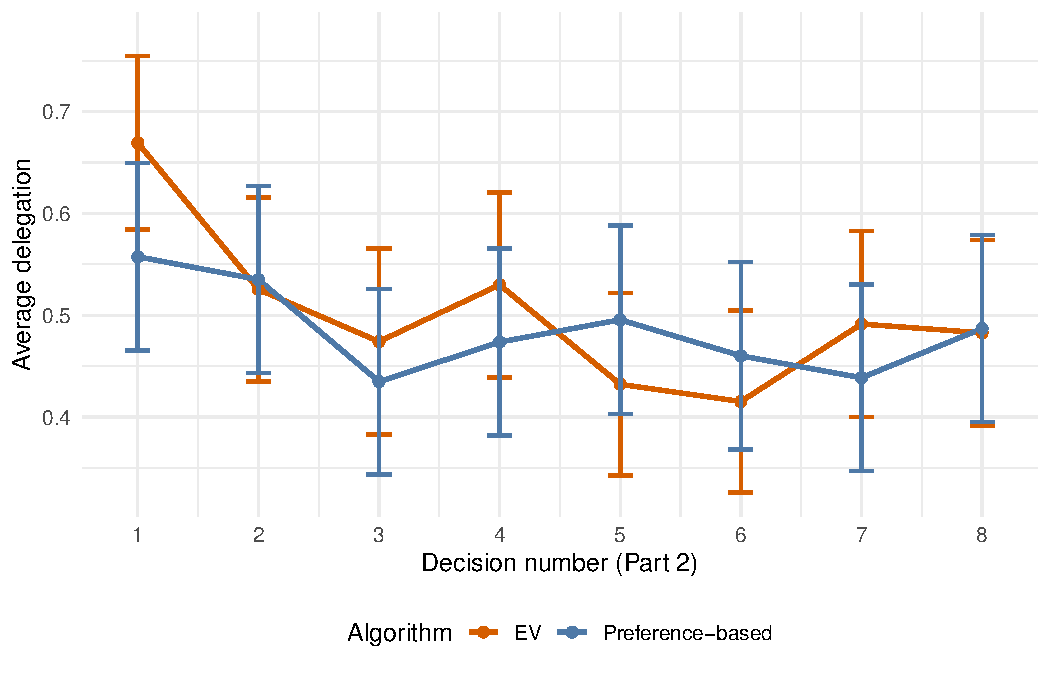
\includegraphics[width=0.8\textwidth]{Figure1_AverageDelegation.pdf}
\caption{Average delegation over decisions in Part 2 by treatment condition.}
\label{fig:average_delegation_over_time}
\end{figure}

\begin{figure}[htbp]
\centering
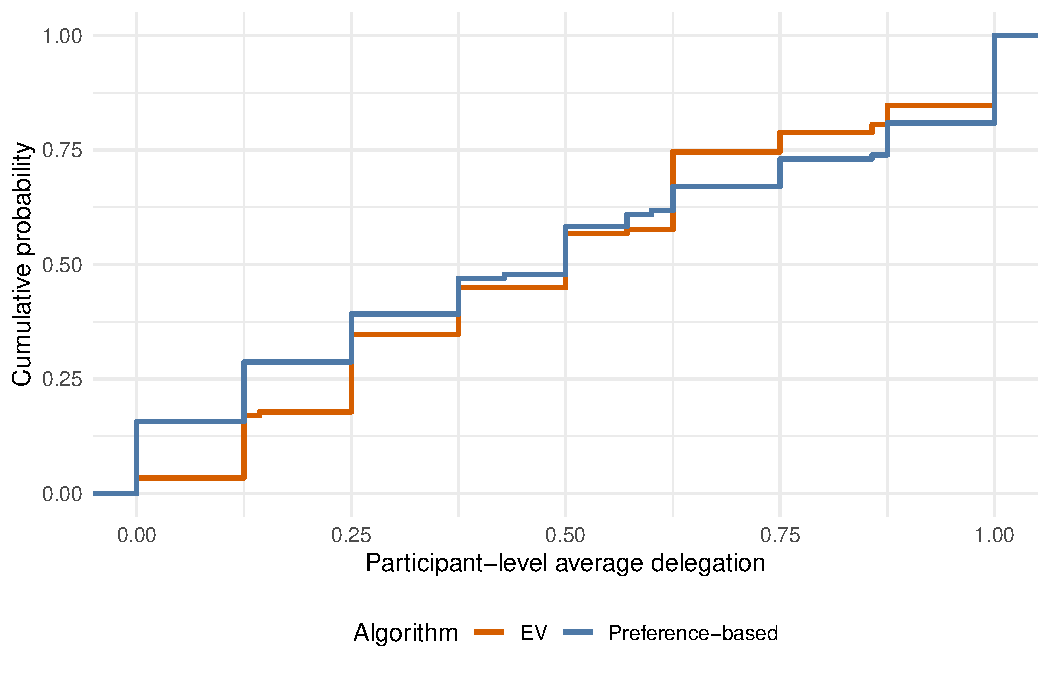
\includegraphics[width=0.78\textwidth]{Figure3_ECDF.pdf}
\caption{ECDF of participant-level average delegation by treatment condition.}
\label{fig:delegation_ecdf}
\end{figure}

\begin{figure}[htbp]
\centering
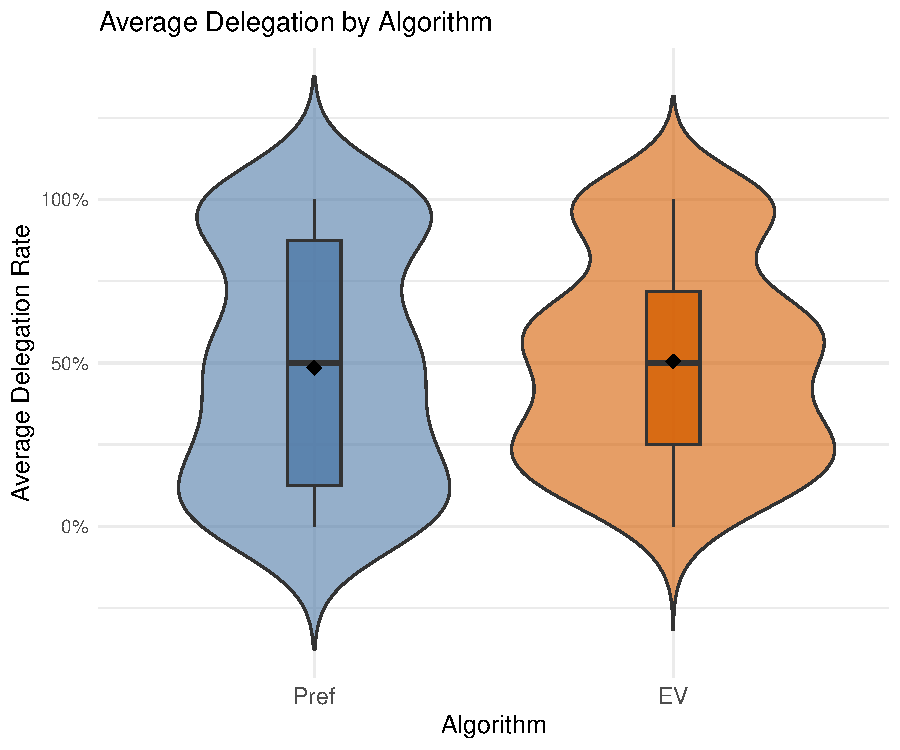
\includegraphics[width=0.78\textwidth]{Figure2_DistributionDelegation.pdf}
\caption{Distribution of delegation propensities across participants.}
\label{fig:delegation_distribution}
\end{figure}

\begin{figure}[htbp]
\centering
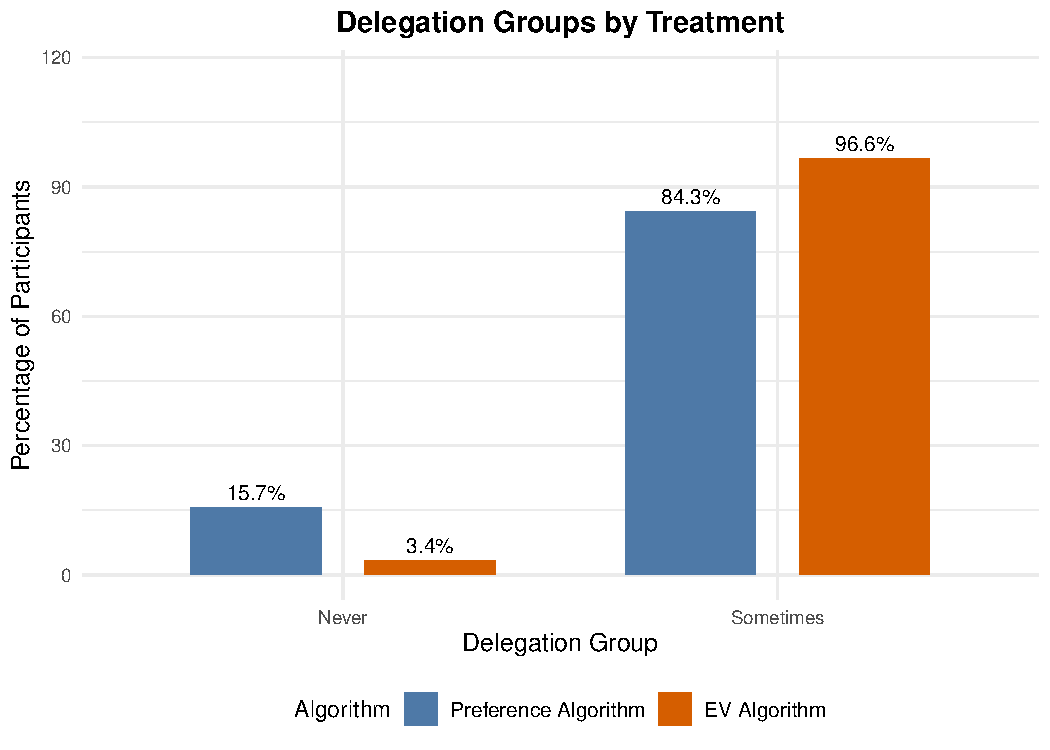
\includegraphics[width=0.78\textwidth]{Figure4_DelegationGroups.pdf}
\caption{Delegation group profiles (never delegators vs. delegators).}
\label{fig:delegation_groups}
\end{figure}

\begin{figure}[htbp]
\centering
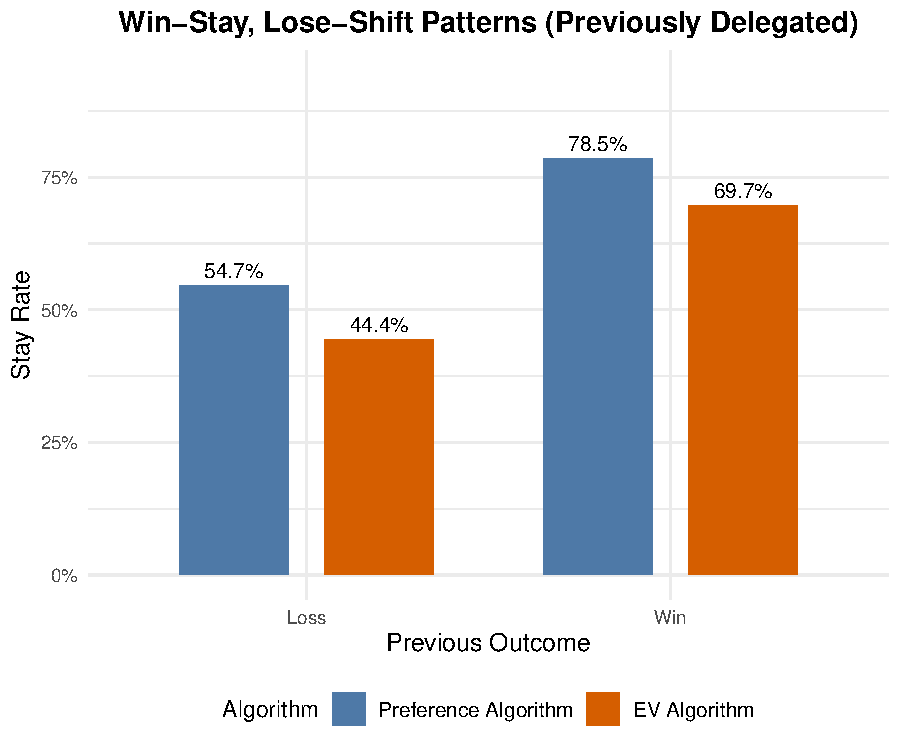
\includegraphics[width=0.8\textwidth]{Figure5_WinStayLoseShift.pdf}
\caption{Win-stay/lose-shift behavior by treatment condition.}
\label{fig:winstay_loseshift}
\end{figure}

\section{Discussion}
\label{sec:discussion}

\subsection{Main takeaway}
This preregistered study shows that preference-based personalization can deter delegation rather than increase it. The deterrence appears in two forms: lower delegation at first contact and a larger subgroup of participants who never delegate under personalization.

The first-contact finding is theoretically important because it captures behavior before participants can learn from repeated outcome feedback. At that stage, delegation is driven primarily by how participants interpret the algorithmic rule itself. Our evidence is consistent with the interpretation that an impersonal EV rule is initially easier to accept as a legitimate external computation than a profile-based personalized rule that is more self-referential.

\subsection{Interpretation in relation to prior work}
The results refine the algorithm aversion/appreciation literature by moving beyond the human-versus-algorithm comparison and focusing on differences between algorithmic decision rules. Our design isolates a contrast in perceived objectivity and self-relevance, which helps explain why personalization can be normatively appealing yet behaviorally resisted.

The non-delegator pattern is especially informative because aggregate means alone would understate it. A sizable share of the treatment contrast is carried by participants who opt out of delegation entirely when personalization is preference-based, consistent with recent work emphasizing autonomy, responsibility, and control as key moderators of algorithm acceptance. At the same time, the mechanism remains inferential in the present design, because these constructs were not directly manipulated.

\subsection{Limitations}
Several limitations should be noted. First, the study is an online experiment with stylized financial lotteries, so external validity to field settings should be interpreted cautiously. Second, although behavioral outcomes are well suited for studying reliance, the design does not directly identify the full psychological mechanism behind first-contact hesitation (e.g., perceived objectivity, profiling concerns, or accountability salience). Third, the present analyses focus on short-run repeated interaction; longer-run adaptation to personalized systems remains an open question.

\subsection{Implications and future research}
For design, the results imply that personalization should not be treated as a uniformly beneficial acceptance lever. In settings where objective criteria are salient and normatively legitimate, objective optimization may face lower initial resistance than preference-based personalization. This has direct implications for the design and communication of decision aids in finance and other high-stakes domains.

Future research should test mechanism-targeted interventions at first contact, including reframing of personalization logic, responsibility framing, and alternative explanation formats. It should also examine whether the non-delegator subgroup is stable across domains, stakes, and cultural contexts.

\subsection{Contributions}
This paper contributes in three ways. First, it provides preregistered evidence that personalization can reduce, rather than increase, delegation at first contact. Second, it shows that resistance is not only transient: personalization is associated with substantially more categorical non-delegation. Third, by comparing two algorithmic decision rules within the same task, it clarifies that behavioral uptake depends on perceived rule characteristics, not only on whether advice is algorithmic.

\subsection{Data and code availability}
Data, analysis code, and study materials will be deposited in a public repository upon acceptance/publication of this manuscript. During peer review, the replication package is maintained in a private repository and will be unblinded and made publicly accessible after acceptance.


\newpage
\thispagestyle{plain}
\addtolength{\topmargin}{-.5cm}
\addtolength{\textheight}{.8cm}

%% \begin{appendices}
% % {\startsupplement
% \renewcommand{\thesection}{Appendix \Alph{section}}
%\renewcommand{\thesubsection}{%\Alph{section}.
%\Roman{subsection}}
%\renewcommand{\thefigure}{}%\Alph{section}.\arabic{figure}}% \Alph{section}}
%\renewcommand{\thetable}{\Alph{section}.\arabic{table}}
%\setcounter{section}{1}
%\setcounter{figure}{0}
%\thispagestyle{plain}

\bibliographystyle{apalike}
\bibliography{library}
 \end{document}
